\documentclass[slidestop,compress,red,mathserif]{beamer}

\usepackage{pgf,pgfarrows,pgfnodes,pgfautomata,pgfheaps,pgfshade}
\usepackage{amsmath,amssymb}
\usepackage{comment}
\usepackage{graphicx}
\usepackage[english]{babel}
\usepackage{tabularx}
\usepackage{xcolor}
\usepackage{multirow}
\usepackage{marvosym}
\usepackage{natbib}
\usepackage{ulem}
\usepackage{wasysym}
\AtBeginDocument{%
  \hypersetup{
    citecolor=Violet,
    linkcolor=Red,   
    urlcolor=Magenta}}

\definecolor{maroon}{rgb}{0.5, 0.0, 0.0}
\definecolor{sangria}{rgb}{0.57, 0.0, 0.04}
\newcommand{\colorcite}[1]{\colorlet{saved}{.}\color{sangria}\cite{#1}\color{saved}}

\setbeamersize{text margin left=6mm, text margin right=2mm}

\mode<presentation>
{
\usetheme{Ilmenau}
\setbeamercovered{transparent}
}

\usecolortheme{default}

\beamertemplateballitem
%\setbeamertemplate{footline}{\insertframenumber/\inserttotalframenumber}

\defbeamertemplate*{footline}{shadow theme}
{%
  \leavevmode%
  \hbox{\begin{beamercolorbox}[wd=2.\paperwidth,ht=2.5ex,dp=1.125ex,leftskip=.3cm plus1fil,rightskip=.3cm]{author in head/foot}%
    \usebeamerfont{author in head/foot}\insertframenumber\,/\,\inserttotalframenumber\hfill%\insertshortauthor
  \end{beamercolorbox}%
  \begin{beamercolorbox}[wd=.5\paperwidth,ht=2.5ex,dp=1.125ex,leftskip=.3cm,rightskip=.3cm plus1fil]{title in head/foot}%
    \usebeamerfont{title in head/foot}%\insertshorttitle%
  \end{beamercolorbox}}%
  \vskip0pt%
}

% number sets
\def\N{\hbox{I \kern-.5em N}}
\def\R{\hbox{I \kern-.5em R}}
\def\Q{\hbox{\hspace*{.25em}{\sf I} \kern-.83em Q}}
\def\T{\rm T}  %%%%  \rm pour roman (ecriture normale)
\def\Z{\rm Z}
\def\ZZ{\hbox{\sf  Z \kern-.8em Z}}
\def \Zplus        {\ZZ^{+}}
\def \bigm {\textsc{penal}}
\def \dst {\textsc{dst}}
\def \src {\textsc{src}}
\def \zlp {z^{\star}_{\textsc{lp}}}
\def \zilp {{\tilde z}_{\textsc{ilp}}}
\def \l    {\textnormal{\textsc{l}}}
\def \Gp   {G_{\textsc{p}}}
\def \Gl   {G_{\l}}
\def \Vp   {V_{\textsc{p}}}
\def \Vl   {V_{\l}}
\def \Ep   {E_{\textsc{p}}}
\def \El   {E_{\l}}
\def \cost {\textsc{cost}}
\def \srlg {\textsc{srlg}}

% number sets
\def \best {\textsc{best}}
\def  \N            {\hbox{I \kern-.5em N}}
\def \RR {\mathbb{R}}
\def \Rplus {\RR^+}
\def  \Z            {\rm Z}
\def  \Zplus        {\Z^+}
\def  \Zplusn       {\Zplus_n}
\def  \ZZ           {\hbox{\sf  Z \kern-.8em Z}}
\def \Z {\mathbb{Z}}

\logo{%
    
\includegraphics[width=2.cm,keepaspectratio]{Figures/ConULogo_CMYK.eps}~%
}

\title[My Title]{High-Resolution Road Vehicle Collision Prediction
for the City of Montreal}
\author[My~Name]{\small
\textbf{Antoine H\'ebert, Timoth\'ee Gu\'edon, Tristan Glatard, Brigitte Jaumard}}
\institute[My Institute/company]
{Concordia University \\ Department of Computer Science and Software Engineering}
\date[]{December 12, 2019}

\begin{document}

\begin{frame} % Cover slide
\titlepage
\end{frame}

%-------------------------------------------------
\section{Introduction}
%-------------------------------------------------

% -------------------------------------------------------------------------------------------------------------------

\begin{frame}
\frametitle{Road accident prediction}
\vfill
\begin{itemize}
\item[] \textbf{Motivation}
  \begin{itemize}
    \item Road accidents result in millions of deaths worldwide every year.
		\item Human and economic impact on society.
  \end{itemize}

\item[] \textbf{Goal:} Estimate the risk of accident at a high-resolution:
  \begin{itemize}
    \item On any road segment
    \item Every hour
  \end{itemize}
\item[] \textbf{Method:}
  \begin{itemize}
    \item Combine several \underline{open datasets} to obtain relevant features
    \item Develop an \underline{accident prediction model} using tree-based algorithms
  \end{itemize}
\end{itemize}
\vfill
\end{frame}

% -------------------------------------------------------------------------------------------------------------------
\begin{frame}{Related work on accident prediction}
    \vfill
  \begin{itemize}
    \item Extensively studied in the last decade
    \item Some studies use small datasets and focus on particular roads \\
        (\colorcite{Chang2005}, \colorcite{Lin2015}, \colorcite{Theofilatos2017})
    \item More recently, some studies cover larger areas but with a coarse resolution
        (\colorcite{Chen2016}, \colorcite{Yuan2018})
    \item Hard to compare performances: only accuracy reported, some study use regression of the risk with various definitions of risk
  \end{itemize}
  \vfill
\end{frame}


\begin{frame}
\frametitle{Open Datasets}

\begin{footnotesize}
We used open datasets provided by the Government of Canada and the City of Montreal.

\begin{itemize}
\item[] \textbf{\href{http://donnees.ville.montreal.qc.ca/dataset/collisions-routieres}{Road collisions Montreal}}
  \begin{itemize}
  	\item Vehicle collisions reported by the police from 2012 to 2017 in Montreal.
  	\item Date and time, severity, localization, etc.
  	\item 134 thousands usable accidents.
  \end{itemize}
\item[] \textbf{\href{https://open.canada.ca/data/en/dataset/3d282116-e556-400c-9306-ca1a3cada77f}{National Road Network}}
  \begin{itemize}
    \item High-resolution information about road segments.
    \item 44 thousands road segments, average length of 124m.
  \end{itemize}
\item[] \textbf{\href{https://climate.weather.gc.ca}{Historical Climate Data}}
  \begin{itemize}
    \item Temperature, humidity, wind speed and direction, visibility, etc. 
    \item At different weather stations in Montreal.
  \end{itemize}
\end{itemize}

\end{footnotesize}

\end{frame}

\begin{frame}
  \frametitle{Table of Contents}
  \tableofcontents
\end{frame}


%-------------------------------------------------
\section{Data preparation}
%-------------------------------------------------

\begin{frame}
	\frametitle{Generating the examples}
	\vfill
	\vfill
  \begin{itemize}
  \item[] \textbf{Positive samples}
    \begin{itemize}
      \item For each accident, identification of the road segment
      \item Using distance between road segments and accidents GPS position.
    \end{itemize}
  \item[] \textbf{Negative samples}
    \begin{itemize}
      \item Every road segment and hour without accident
      \item 2 billion negative examples $\Rightarrow$ too many to work with
      \item Use a subsample of all possible negative samples (0.1\%).
    \end{itemize}
  \vfill
  \item[] $\Rightarrow$ 2 million negative samples for about 135,000 positive samples.
    \end{itemize}
  \vfill
  \vfill
\end{frame}

\begin{frame}
	\frametitle{Feature creation}
	\vfill
	\begin{itemize}
    \item[] \textbf{Weather}
    \begin{itemize}
      \item Interpolation of weather statistics  between several stations
      \item Used a moving average for atmospheric phenomenons
    \end{itemize}
    \item[] \textbf{Road segment}
    \begin{itemize}
      \item Length of each road segment
      \item Type of road (highway, street, boulevard, etc)
      \item Number of accidents on the road segment during 4 previous years
    \end{itemize}
    \item[] \textbf{Date and time} \begin{itemize}
      \item \href{https://miro.medium.com/max/515/1*70cevmU8wNggGJEdLam1lw.png}{Cyclic features}: hour of the day, day of the month
      \item Day of week
      \item Solar elevation
    \end{itemize}
	\end{itemize}
	\vfill
\end{frame}

\begin{frame}
  \frametitle{Infrastructure}
  \begin{columns}
  \begin{column}{0.6\textwidth}
  \begin{itemize}
    \item \textbf{Apache Spark} \colorcite{zaharia2010spark}       
    \begin{itemize}
    \item Parallel computing, in-memory, data locality, lazy evaluation
    \item Used the DataFrame API
    \end{itemize}
    \item \textbf{Compute Canada cluster}
    \begin{itemize}
      \item Used about 2 CPU years
      \item Pre-processing reduced to a few hours
    \end{itemize}
  \end{itemize}
  \end{column}
\begin{column}{0.4\textwidth}
  \begin{itemize}
  \item[] 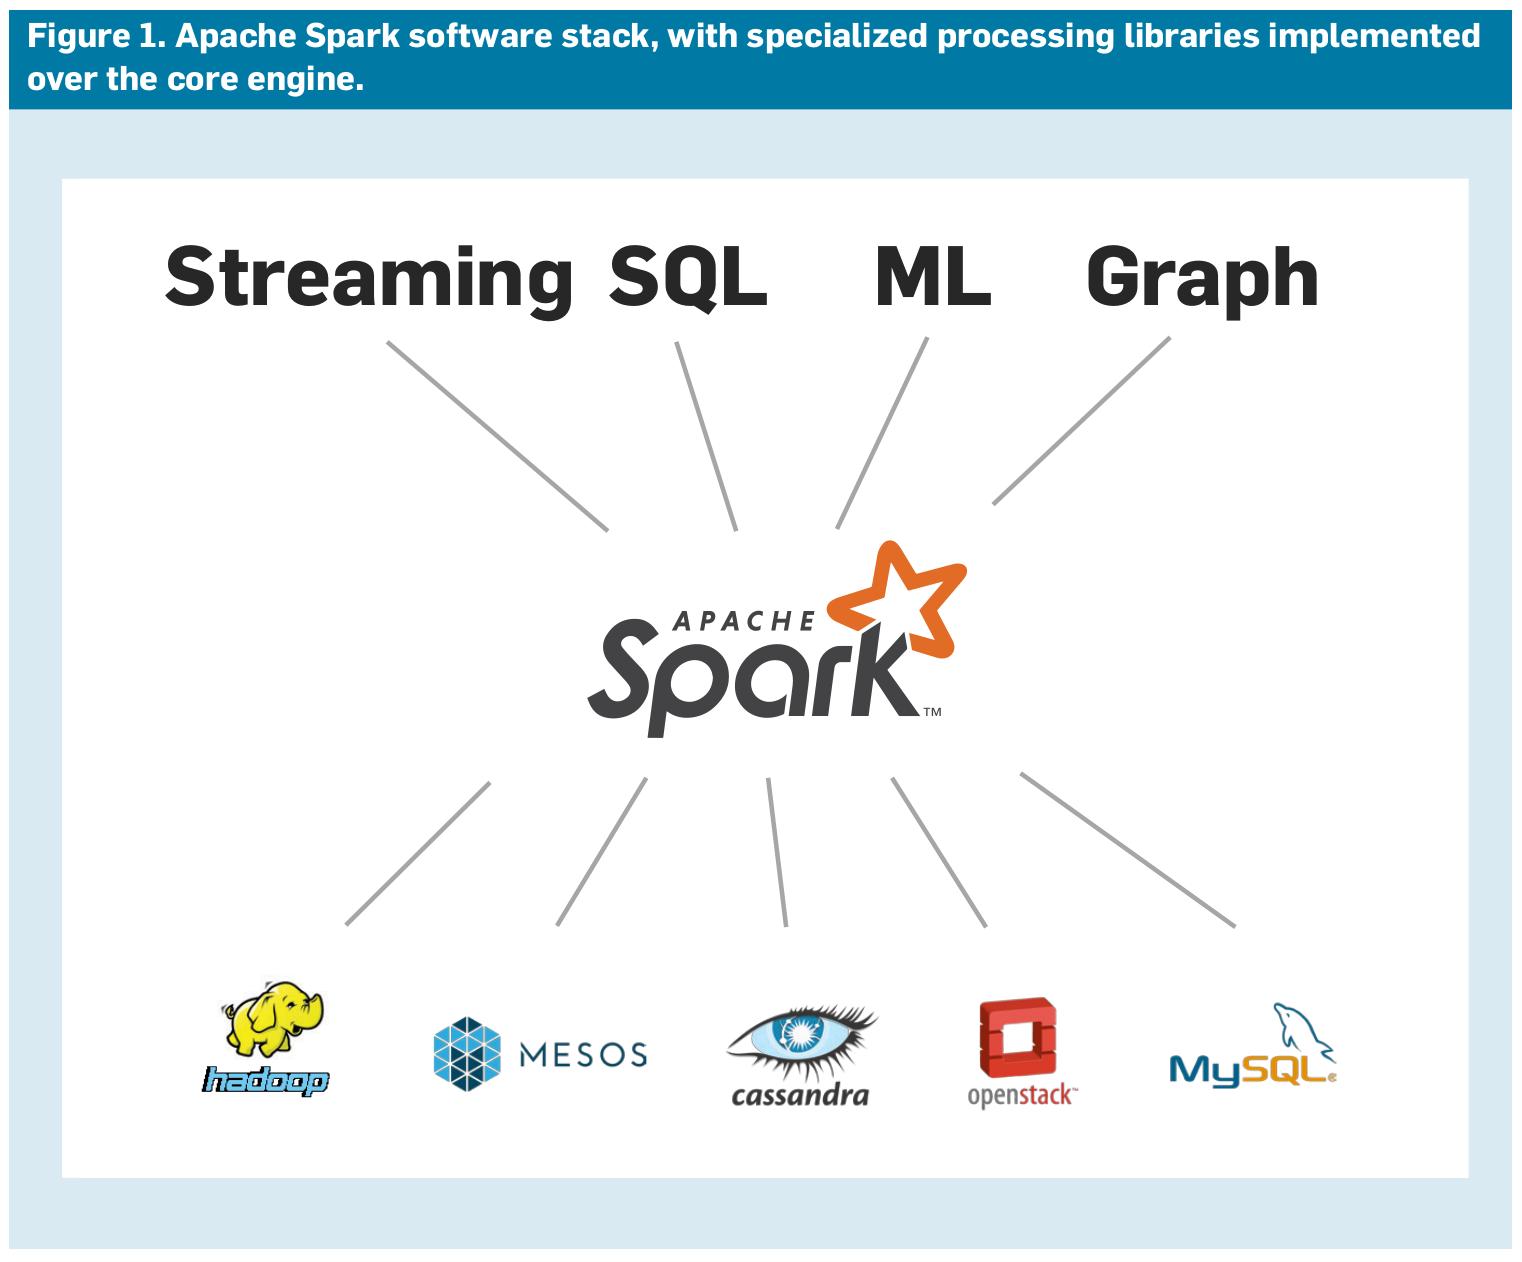
\includegraphics[height=3cm, keepaspectratio]{Figures/spark.png}
  %\vspace{0.5cm}
  \item[] 
\includegraphics[height=3cm, keepaspectratio]{Figures/cc-logo.png}
  \end{itemize}
\end{column}
\end{columns}
\end{frame}


%-------------------------------------------------
\section{Methods}
%-------------------------------------------------


\begin{frame}
\frametitle{Tree-based classification algorithms}
\begin{itemize}
\vfill
\item[] \textbf{Selected algorithms:} Tree-based algorithms
  \begin{itemize}
  	\item Random Forest
    \item Balanced Random Forest (\colorcite{Chen2004})
    \item Gradient Boosted Trees (GBT) - XGBoost implementation
  \end{itemize}
\vfill
\end{itemize}
\end{frame}

% -------------------------------------------------------------------------------------------------------------------

\begin{frame}
\frametitle{Dealing with data imbalance (\cite{Chen2004})}
\begin{itemize}
  \item[] \textbf{Weighted Random Forests (WRF)}
    \begin{itemize}
      \item Add weights to the classes when growing the tree.
      \item Add weights to the classes at the voting time.
    \end{itemize}

  \item[] \textbf{Balanced Random Forests (BRF)}
    \begin{itemize}
      \item Combine undersampling and ensemble method.
      \item For each tree: randomly draw a balanced sample.
      \item The rest of the algorithm is identical to Random Forests.
    \end{itemize}

  \item[] \textbf{BRF versus WRF}
    \begin{itemize}
      \item No clear winner in terms of prediction power! But...
      \item WRF - More vulnerable to noise on minority class
      \item BRF - More computationally efficient
      \item BRF - Easier to implement in Apache Spark
    \end{itemize}
\end{itemize}
\end{frame}


\begin{frame}
\frametitle{Implementation of BRF in Apache Spark}
\begin{itemize}
    \vfill
    \item[] \textbf{In random forest implementation}: 
        \begin{itemize}
            \item $m_i$ the number of times an example appears in the sample of a tree
            \item $m_i \thicksim \textit{Poisson}(\lambda)$
        \end{itemize}
    \item[] \textbf{Modification:} two different Poisson distributions:
        \begin{itemize}
            \item For positive samples: $m_i \thicksim \textit{Poisson}(\lambda_p)$
            \item For negative samples: $m_i \thicksim \textit{Poisson}(\lambda_n)$
            \item $\lambda_p < \lambda_n$
        \end{itemize}
    \vfill
\end{itemize}
\end{frame}

\begin{frame}
\frametitle{Experimentation with our BRF implementation}
\begin{itemize}
  \item Dataset from the imbalanced-learn library (\colorcite{Woods1993})
  \item Same behavior between the two implementations
  \item BRF does not perform better on this dataset
\end{itemize}

\centering
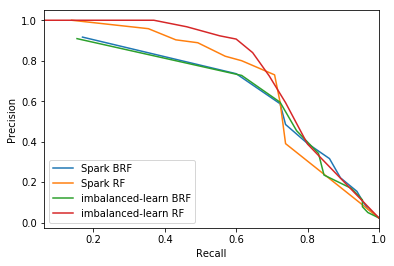
\includegraphics[height=3.0cm, keepaspectratio]{Figures/test_brf_pr.png}\\
$\mathrm{Recall} = \frac{TP}{TP+FN} \quad  \mathrm{Precision} = \frac{TP}{TP+FP}$

\end{frame}

%-------------------------------------------------
\section{Results}
%-------------------------------------------------

\begin{frame}
	\frametitle{Results: PR curves}
	\begin{itemize}
		\item Results are much better than the baseline
		\item No significant difference between the BRF and RF
	\end{itemize}
\centering
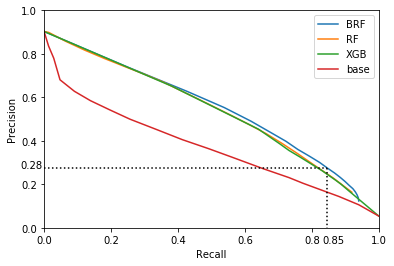
\includegraphics[height=4cm, keepaspectratio]{Figures/pr.png}
\begin{equation*}
  \mathrm{Recall} = \frac{TP}{TP+FN} \quad  \mathrm{Precision} = \frac{TP}{TP+FP}
\end{equation*}
\end{frame}

\begin{frame}
	\frametitle{Results: ROC curves}
	\begin{itemize}
     \item We can identify 85\% of the accidents with a false positive rate of 13\%
	\end{itemize}
\centering
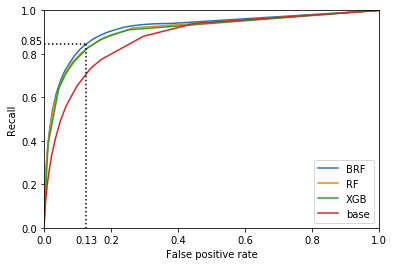
\includegraphics[height=4cm, keepaspectratio]{Figures/roc.png}
\hspace*{-1cm}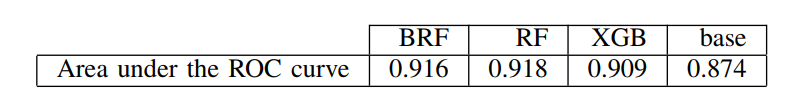
\includegraphics[height=1.5cm, keepaspectratio]{Figures/results_table.png}
\end{frame}

\begin{frame}
	\frametitle{Results}
	\begin{itemize}
		\item Despite similar PR curves, when the same decision threshold is used, BRF and RF obtain very different results 
	\end{itemize}
\centering
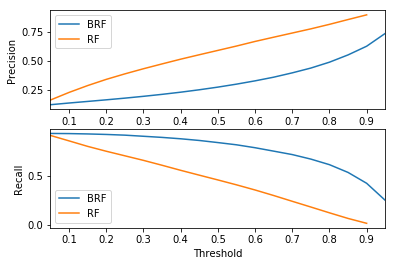
\includegraphics[height=4cm, keepaspectratio]{Figures/pr_threshold.png}
\end{frame}

\begin{frame}
	\frametitle{Feature Importance}
\centering
\hspace*{-2cm} Using mean decrease in entropy (\cite{louppe2013understanding}) \\
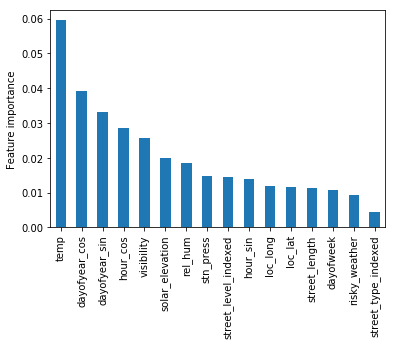
\includegraphics[height=5cm, keepaspectratio]{Figures/features.png} \\
\hspace*{-2cm} Most important feature: previous accident count (67\%)

\end{frame}

%-------------------------------------------------
\section{Conclusion}
%-------------------------------------------------

\begin{frame}
  \frametitle{Conclusion}
  \begin{itemize}
    \item[] \textbf{Results}
    \begin{itemize} 
    \item We can identify 85\% of the accidents with a false positive rate of 13\%
    \item Model works at a resolution of 1 hour, between each intersection
    \item $\Rightarrow$ take security measures at specific road segment and times
    \end{itemize}
    \item[] \textbf{Usability}
    \begin{itemize} 
    \item Reproducible for other cities: only simple datasets were used
    \item Code is available at \url{https://github.com/big-data-lab-team/accident-prediction-montreal}
    \end{itemize}
  \end{itemize}
  \centering
  
\includegraphics[height=2cm]{Figures/github.png}
\end{frame}

\begin{frame}
  \frametitle{Future work}
  \begin{itemize}
    \item Analyse why BRF did not perform better than RF
    \item Add more datasets: traffic, construction, population density
    \item Experiment with different types of algorithms (DNN) and data imbalance techniques (SMOTE, focal loss, etc)
  \end{itemize}
  \centering
  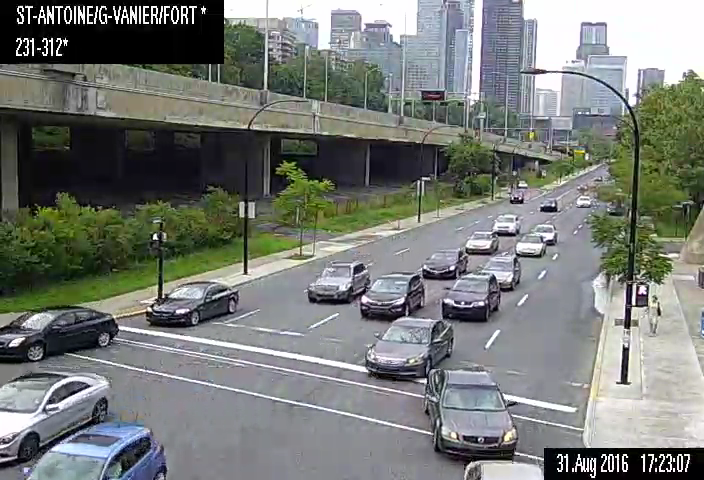
\includegraphics[height=4cm]{Figures/traffic_camera.png}
\end{frame}

% \begin{frame}
%   \vspace{2cm}
%   \centering
%   {\Large \textbf{MERCI !}}

% \end{frame}

% -------------------------------------------------------------------------------------------------------------------------
% -------------------------------------------------------------------------------------------------------------------------
%% -------------------------------------------------------------------------------------------------------------------------

\begin{frame}[allowframebreaks]
\frametitle{References}

{\scriptsize

\bibliographystyle{plainnat}
\bibliography{Biblio}

}


\end{frame}

\end{document}
